% 6-page A4 conference version (IEEE two-column, 10 pt Times). Blind: no author, affiliation, e-mail or repository link.
% Numbers come from ../paper/numbers.tex (generated by analysis/paper/make_numbers.py); figures from ../data/figures, used as generated: phase1/phase1_accuracy.png, phase2/algorithms/*.png, phase2/timer_vs_counter/circuit/*.png, phase4/algorithms/*.png, phase4/all_boards_all_circuits.png.
% Build: make paper-6p
\documentclass[conference,a4paper,10pt]{IEEEtran}
\usepackage{booktabs,graphicx,amsmath,xspace,microtype}
\usepackage{iftex}
\ifXeTeX\usepackage{fontspec}
\setmainfont{Times New Roman}
\setmonofont{Courier New}[Scale=MatchLowercase]\fi
\usepackage[hidelinks]{hyperref}
% generated by analysis/paper/make_numbers.py -- do not edit
\newcommand{\ACallEspLo}{8.4}
\newcommand{\AerMax}{$6.2\times10^{-11}$}
\newcommand{\AerMaxN}{12}
\newcommand{\AmpBytes}{8}
\newcommand{\ApbMHz}{80}
\newcommand{\BaudSp}{115\,200}
\newcommand{\BitsPerByte}{10}
\newcommand{\CnotEspLo}{0.0522}
\newcommand{\CondCap}{$10^{4}$}
\newcommand{\CondMaxTwo}{4.7}
\newcommand{\ConstRelErr}{$1.71\times10^{-8}$}
\newcommand{\CounterTickNs}{12.5}
\newcommand{\CrossBelow}{1}
\newcommand{\CrossBoth}{10}
\newcommand{\CrossNone}{1}
\newcommand{\CyclesCnotEspHi}{22}
\newcommand{\CyclesCnotEspLo}{4.18}
\newcommand{\CyclesCphaseEspHi}{12}
\newcommand{\CyclesHEspHi}{19}
\newcommand{\DirFourteen}{$1.7\times10^{-2}$}
\newcommand{\DirMaxTwelve}{$5.5\times10^{-5}$}
\newcommand{\DirThirteen}{$1.1\times10^{-3}$}
\newcommand{\DoubleMax}{$8.5\times10^{-9}$}
\newcommand{\DupNineIndep}{15}
\newcommand{\DupNineRows}{100}
\newcommand{\DupTenIndep}{29}
\newcommand{\EspHiLongest}{529}
\newcommand{\EspHiWorstPct}{0.85}
\newcommand{\EspResUs}{1}
\newcommand{\FcpuEspHi}{240}
\newcommand{\FcpuEspLo}{80}
\newcommand{\FcpuUno}{16}
\newcommand{\FloorMsEspHi}{6.8}
\newcommand{\FloorMsEspLo}{3.7}
\newcommand{\FloorMsUno}{3.4}
\newcommand{\GateCrossAll}{52}
\newcommand{\GateCrossN}{52}
\newcommand{\GateSeqGrover}{8}
\newcommand{\GateSeqMax}{7}
\newcommand{\GroverLastMinEspHi}{75}
\newcommand{\GroverLastMinEspLo}{28}
\newcommand{\GroverLastNEspHi}{12}
\newcommand{\GroverLastNEspLo}{10}
\newcommand{\GroverLastRepsEspHi}{1}
\newcommand{\GroverLastRepsEspLo}{4}
\newcommand{\GroverNineSessions}{3}
\newcommand{\GroverNineSimHi}{8.8}
\newcommand{\GroverNineSimLo}{4.1}
\newcommand{\GroverPredEspHi}{13}
\newcommand{\GroverPredEspLo}{12}
\newcommand{\GroverTwelveNH}{3\,940\,012}
\newcommand{\GroverTwelvePm}{0.89}
\newcommand{\GroverTwelveRaw}{0.109}
\newcommand{\IdBoardsFour}{ESP32, ESP8266}
\newcommand{\IdBoardsThree}{ESP32, ESP8266}
\newcommand{\IdBoardsTwo}{ESP32, ESP8266, Uno}
\newcommand{\IqrOver}{60}
\newcommand{\IqrThresh}{20}
\newcommand{\KMaxN}{22}
\newcommand{\LabNoise}{10}
\newcommand{\LabWeak}{4}
\newcommand{\LogLossFourteen}{1.25}
\newcommand{\LogLossHi}{1.17}
\newcommand{\LogLossLo}{1.16}
\newcommand{\LogLossOverPct}{16}
\newcommand{\MapeDecTwoClean}{16.5}
\newcommand{\MapeOne}{47}
\newcommand{\MapeOneCOne}{28}
\newcommand{\MapeOneClean}{46}
\newcommand{\MapeOneEspHi}{26}
\newcommand{\MapeOneEspLo}{67}
\newcommand{\MapeOneUno}{45}
\newcommand{\MapeTwo}{17}
\newcommand{\MapeTwoClean}{17}
\newcommand{\MapeTwoEspHi}{6}
\newcommand{\MapeTwoEspHiClean}{6}
\newcommand{\MapeTwoEspLo}{17}
\newcommand{\MapeTwoEspLoClean}{15}
\newcommand{\MapeTwoG}{14}
\newcommand{\MapeTwoIdent}{12.4}
\newcommand{\MapeTwoUno}{25}
\newcommand{\MapeTwoUnoClean}{25}
\newcommand{\MapeTwoUnoQft}{71}
\newcommand{\MemBEspHi}{110\,580}
\newcommand{\MemBEspHiTotal}{256\,328}
\newcommand{\MemOkEspHi}{13}
\newcommand{\MemOkEspLo}{12}
\newcommand{\MemOkUno}{7}
\newcommand{\MemOverheadUnoMax}{206}
\newcommand{\MemOverheadUnoMin}{200}
\newcommand{\MemPredEspHi}{13}
\newcommand{\MemPredEspHiTotal}{14}
\newcommand{\MemPredEspLo}{12}
\newcommand{\MemPredUno}{7}
\newcommand{\MemSramUno}{2\,048}
\newcommand{\MemStateAtWallEspHi}{131\,072}
\newcommand{\MemWallEspHi}{14}
\newcommand{\MemWallEspLo}{13}
\newcommand{\MemWallRows}{9}
\newcommand{\MemWallUno}{8}
\newcommand{\MixedPoints}{0}
\newcommand{\ModelFloorUs}{100}
\newcommand{\NCOne}{30}
\newcommand{\NCleanTwo}{30}
\newcommand{\NCross}{12}
\newcommand{\NOffPoints}{124}
\newcommand{\NSessions}{70}
\newcommand{\NTestTwo}{32}
\newcommand{\NTwoIdent}{20}
\newcommand{\NWeakTwo}{36}
\newcommand{\NormPerH}{$3.42\times10^{-8}$}
\newcommand{\OffNMaxEspHi}{14}
\newcommand{\OffNMaxEspLo}{13}
\newcommand{\OffNMaxUno}{8}
\newcommand{\PointCapH}{2}
\newcommand{\PoneDirFirstFail}{13}
\newcommand{\PoneDirLastPass}{12}
\newcommand{\PoneDirLastPassHi}{13}
\newcommand{\PoneDirLastPassLo}{12}
\newcommand{\PoneGate}{$10^{-3}$}
\newcommand{\PoneGroverFirstFail}{9}
\newcommand{\PoneGroverLastPass}{8}
\newcommand{\PoneGroverLastPassHi}{10}
\newcommand{\PoneGroverLastPassLo}{7}
\newcommand{\PoneGroverMaxPass}{$3.61\times10^{-4}$}
\newcommand{\PoneMaxBell}{$3.45\times10^{-8}$}
\newcommand{\PoneMaxHall}{$2.43\times10^{-7}$}
\newcommand{\PoneMaxQft}{$2.43\times10^{-7}$}
\newcommand{\PoneThreshHi}{$10^{-2}$}
\newcommand{\PoneThreshLo}{$10^{-4}$}
\newcommand{\PrevMoneEspHi}{21.0}
\newcommand{\PrevMtwoEspLo}{23.0}
\newcommand{\ProvCommitted}{69}
\newcommand{\ProvDirty}{70}
\newcommand{\ProvUncommitted}{1}
\newcommand{\PyVer}{3.11.7}
\newcommand{\RFiveHi}{2.0}
\newcommand{\RFiveLo}{0.5}
\newcommand{\RFiveMs}{1}
\newcommand{\RatioLongSEspHi}{0.896}
\newcommand{\RatioLongSEspLo}{2.88}
\newcommand{\RatioLongSUno}{29.8}
\newcommand{\RatioMaxEspLo}{1.0000}
\newcommand{\RatioMaxUno}{0.9951}
\newcommand{\RatioMedEspHi}{0.9995}
\newcommand{\RatioMedEspLo}{0.9974}
\newcommand{\RatioMedUno}{0.9943}
\newcommand{\RatioMinEspLo}{0.9317}
\newcommand{\RatioMinUno}{0.9018}
\newcommand{\RatioNEspHi}{26}
\newcommand{\RatioNEspLo}{24}
\newcommand{\RatioNUno}{19}
\newcommand{\RecordedNEspHi}{50}
\newcommand{\RecordedNEspLo}{45}
\newcommand{\RecordedNUno}{28}
\newcommand{\ReproPthreeE}{14}
\newcommand{\ReproPthreeEMax}{114}
\newcommand{\ReproPthreeN}{45}
\newcommand{\ReproPthreeResid}{96}
\newcommand{\ReproPthreeSim}{21}
\newcommand{\ReproPtwoMaxPct}{0.0056}
\newcommand{\ReproPtwoMedPct}{0.00012}
\newcommand{\ReproPtwoN}{9}
\newcommand{\Reps}{100}
\newcommand{\ReqBytes}{4}
\newcommand{\ResidHi}{3225}
\newcommand{\ResidLo}{535}
\newcommand{\ResidMed}{772}
\newcommand{\RespBytes}{6}
\newcommand{\SelfTestAll}{5}
\newcommand{\SelfTestHi}{2.9}
\newcommand{\SelfTestLo}{2.0}
\newcommand{\SelfTestPass}{5}
\newcommand{\SensOneAllFour}{48.2}
\newcommand{\SensOneAllTwo}{46.4}
\newcommand{\SensTwoAllMax}{17.9}
\newcommand{\SensTwoAllMin}{14.1}
\newcommand{\SensTwoIdentMax}{14.5}
\newcommand{\SensTwoIdentMin}{12.4}
\newcommand{\SimSmallMs}{20}
\newcommand{\SimSpreadAbout}{2}
\newcommand{\SimSpreadMax}{2.92}
\newcommand{\SimSpreadMed}{1.53}
\newcommand{\TMaxDays}{40.7}
\newcommand{\TMaxS}{$3.518\times10^{6}$}
\newcommand{\UnoBelowPct}{0.6}
\newcommand{\UnoResUs}{4}
\newcommand{\UsableNEspHi}{44}
\newcommand{\UsableNEspLo}{29}
\newcommand{\UsableNUno}{19}
\newcommand{\WeakFirst}{ten}
\newcommand{\WeakMin}{30}
\newcommand{\WeakPthreeEspHi}{12,13}
\newcommand{\WeakPtwoEspHi}{9,10,11,12}
\newcommand{\WeakPtwoEspLo}{10}
\newcommand{\WeakSwitchWith}{16.3}
\newcommand{\WeakSwitchWithout}{17.0}
\newcommand{\WireMs}{0.87}
\newcommand{\WrapS}{53.687}

\newcommand{\uno}{Uno\,R3}
\newcommand{\espA}{ESP8266}
\newcommand{\espB}{ESP32}
\newcommand{\cn}[1]{\texttt{#1}}
\newcommand{\hall}{\cn{h\_all}}
\newcommand{\bell}{\cn{bell\_ghz}}
\newcommand{\qft}{\cn{qft}}
\newcommand{\grover}{\cn{grover}}
\newcommand{\us}{\,\textmu s\xspace}

\newcommand{\panel}[2]{\begin{minipage}[t]{0.47\textwidth}\centering\includegraphics[width=\linewidth]{#1}\\[-2pt]\small #2\end{minipage}}
\begin{document}
\title{What Limits Statevector Quantum-Circuit Simulation on Microcontrollers? Memory, Time and Offload on Uno, ESP8266 and ESP32}
\author{\IEEEauthorblockN{Anonymous submission}}
\maketitle
\begin{abstract}
Can a microcontroller simulate a quantum circuit itself, or should it offload the circuit to a PC? We benchmark a float32 statevector simulator on an Arduino \uno, an \espA\ and an \espB\ for four circuits (\hall, \bell, \qft, \grover), measuring memory limits, execution time and a serial offload to Qiskit Aer. For the first three circuits the memory wall lies at $n=\MemWallUno$, \MemWallEspLo\ and \MemWallEspHi\ qubits and is consistent with $\lfloor\log_2(B/8)\rfloor$, where $B$ is the free memory read at $n=2$. A per-gate-kind time model fitted at small $n$ predicts held-out run times with \MapeTwoClean\,\% mean absolute percentage error, against \MapeOneClean\,\% for one constant per board. Offloading overtakes local execution at between $n=\CrossMinN$ and $n=\CrossMaxN$ qubits, depending on board, circuit and PC speed. The study uses one unit per board, one PC and one baud rate, and several analysis rules were set after the data were seen.
\end{abstract}
\begin{IEEEkeywords}
statevector simulation, microcontrollers, memory wall, performance model, computation offloading
\end{IEEEkeywords}

\section{Introduction}
A dense statevector simulation of $n$ qubits stores $2^n$ complex amplitudes~\cite{haener2017}. On a microcontroller the state competes with the program and the runtime for kilobytes of RAM, and the arithmetic runs on 8-bit or soft-float cores. Whether a circuit can be simulated on such a device, and whether it is better sent to a PC, is a practical question for embedded and educational quantum tooling. Statevector simulation on a microcontroller has been shown for a few qubits on an RP2040 board~\cite{carney2023}; a limited literature search found no peer-reviewed study on Arduino or ESP boards. Dense statevector simulators and their exponential memory demand are well documented~\cite{haener2017}, as are CPU and GPU simulators such as Qiskit Aer (cited through the Qiskit paper~\cite{javadiabhari2024}) and fast simulators that trade numerical precision against memory and speed~\cite{yusufov2023}. We claim no novelty over these simulators~\cite{haener2017,javadiabhari2024,yusufov2023} or the textbook circuits we use (QFT~\cite{coppersmith1994}, Grover search~\cite{grover1996}).

We ask: \emph{what limits statevector simulation on microcontrollers, how well can those limits be predicted, and where is the local-versus-offload trade-off?} Contributions: (i) the memory and time limit of each board and circuit, with the evidence type for each; (ii) a memory rule and two time models with held-out scores; (iii) the offload crossover as brackets of measured $n$ under the fastest and slowest PC simulation speed we observed, so the host PC is part of the result. This is a characterisation study, not a pre-registered test: analysis rules were refined while the data were examined, and every such choice is disclosed in Section~\ref{sec:disc}.

\section{System and Method}\label{sec:method}
\textbf{Simulator and circuits.} All boards run the same C++ code: the state is $2^n$ complex float32 amplitudes (\AmpBytes\,B each) and each gate kernel (H, CNOT, controlled-phase CP) sweeps all $2^n$ indices, so the work of a circuit is (gate calls)$\times2^n$. The circuits are \hall\ ($n$ H gates), \bell\ (one H, $n{-}1$ CNOT), \qft\ ($n$ H and $n(n{-}1)/2$ CP) and \grover\ ($\lfloor\frac{\pi}{4}\sqrt{2^n}\rfloor$ iterations of a phase oracle and a diffusion step built from recursively decomposed multi-controlled phase gates). The firmware gate sequence was checked against the PC reference gate by gate for $n\le\GateSeqMax$ (\GateSeqGrover\ for \grover), and the gate counts against counting kernels for \GateCrossN\ of \GateCrossAll\ (circuit, $n$) pairs. Boards: Arduino \uno\ (\FcpuUno\,MHz, \MemSramUno\,B SRAM, static array), NodeMCU \espA\ (\FcpuEspLo\,MHz, no FPU) and \espB\ DevKit (\FcpuEspHi\,MHz, FPU); one unit each. Boards return timing only, never the final state.

\textbf{Phases.} \emph{Phase~1} compares the float32 build on the PC with Qiskit Aer (infidelity). \emph{Phase~2} runs the circuit on the board for $n=2,3,\ldots$ until a memory wall or a per-point time cap (\PointCapH\,h); each point is up to \Reps\ repetitions, reported as the median and interquartile range (IQR) of the \texttt{micros()} time around the circuit call. A wall is recorded only with positive evidence (linker RAM overflow on the Uno, failed allocation on the ESP boards). A second ESP32 timestamps a pin raised around the same call (\CounterTickNs\,ns per tick) as an independent but \emph{uncalibrated} reference: a loopback self-test passed \SelfTestPass\ of \SelfTestAll\ scenarios with a constant offset of \SelfTestLo--\SelfTestHi\,\textmu s, but one crystal generates and measures. A counter value is used only if its pairs pass four validity rules, and rule R5 additionally rejects pairs whose counter/\texttt{micros()} ratio lies outside $[\RFiveLo,\RFiveHi]$ or near the $2^{32}$-tick wrap. \emph{Phase~3} offloads: the board sends a \ReqBytes-byte request (circuit, $n$, CRC-8) at \BaudSp\,baud, the PC re-simulates with Qiskit Aer on every request, draws one outcome and returns a \RespBytes-byte frame; the board times the round trip. It is a latency measurement, not a correctness test. A point with fewer than \WeakMin\ independent repetitions is \emph{weak}: it is never fitted or scored and is drawn hollow. Several points were measured in more than one session; one selector fixes which session is primary evidence, and the others feed only the reproducibility check. The selector was fixed late, after the data and the first scores were known. Firmware versions are classified by their effect on the timed region (class~A: reference; class~B: timing-relevant difference, as for all selected \espA\ \grover\ points, which ran a timer interrupt inside the timed region); points of class~B are not fitted.

\textbf{Memory rule.} The state needs $M(n)=\AmpBytes\cdot2^n$ bytes and fits if $M(n)\le B$:
\begin{equation}\label{eq:mem}n_{\max}=\lfloor\log_2(B/\AmpBytes)\rfloor,\end{equation}
with $B$ read from low-$n$ runs only: the SRAM left after the compiler-reported static use (Uno), the free heap at $n=2$ (\espA) and, on the \espB, the largest free block, since one contiguous allocation is needed.

\textbf{Time models.} With $G_c(n)$ gate calls of circuit $c$ ($G_{\hall}=n$, $G_{\bell}=n$, $G_{\qft}=n+\frac{n(n-1)}{2}$) and $N_{c,k}$ calls of kind $k\in\{\mathrm{H},\mathrm{CNOT},\mathrm{CP}\}$,
\begin{align}
\text{M1:}\ & T_{\mathrm{local}}(n)=c_b\,G_c(n)\,2^n,\label{eq:m1}\\
\text{M2:}\ & T_{\mathrm{local}}(n)=\textstyle\sum_{k}c_{b,k}N_{c,k}(n)\,2^n+a_b\,G_c(n),\label{eq:m2}
\end{align}
with one constant $c_b$ per board (M1), or one non-negative cost per gate kind plus a per-call term, shared by the circuits of a board (M2; non-negative least squares on relative error). Per series the largest three $n$ are held out, every other point with a median of at least \ModelFloorUs\,\textmu s is fitted unless it is weak or class~B, and the score is the mean absolute percentage error
\begin{equation}\label{eq:mape}\mathrm{MAPE}=\frac{100}{N}\sum_{i=1}^{N}\frac{|T^{\mathrm{pred}}_i-T^{\mathrm{meas}}_i|}{T^{\mathrm{meas}}_i}\end{equation}
over the $N$ non-weak held-out points. M1c fits one constant per board and circuit; M2g is M2 fitted without \grover. A fit is called identifiable if it has at least (parameters $+2$) points, full column rank and no coefficient on the non-negativity boundary. For \grover, $G_{\grover}=n+k(n)\bigl(16\cdot3^{\,n-3}+8n-6\bigr)$ for $n\ge3$, with $k(n)=\max(\lfloor\frac{\pi}{4}\sqrt{2^n}\rfloor,1)$ evaluated in float32 as in the firmware, and the reference marked-state probability is $P_{\mathrm{marked}}=\sin^2\bigl((2k+1)\theta\bigr)$ with $\theta=\arcsin 2^{-n/2}$.

\textbf{Offload and crossover.} The round trip of one request is
\begin{equation}\label{eq:off}T_{\mathrm{off}}(n)=T_{\mathrm{wire}}+T_{\mathrm{res},b}(n)+T_{\mathrm{pc},c}(n),\end{equation}
the serial wire time $T_{\mathrm{wire}}=\BitsPerByte\,(\ReqBytes+\RespBytes)/\mathrm{baud}$ (\WireMs\,ms), a board-and-link residual (board compute, USB-serial latency, host scheduling; per point, the round-trip median minus the simulation median minus the wire time) and the PC simulation time (Aer build, run and sample, logged per point). $T_{\mathrm{pc}}$ is a range: the fastest and slowest value observed over all Phase~3 sessions give a ``fast'' and a ``slow'' PC bound. The crossover
\begin{equation}\label{eq:cross}n^{*}=\min\{n:\ T_{\mathrm{off}}(m)<T_{\mathrm{local}}(m)\ \ \forall\,m\ge n\text{ measured}\}\end{equation}
is reported as a bracket of two consecutive measured $n$ for each bound, without interpolation.

\section{Results}\label{sec:results}
\begin{figure*}[t]
\centering
\begin{minipage}[t]{0.47\textwidth}\centering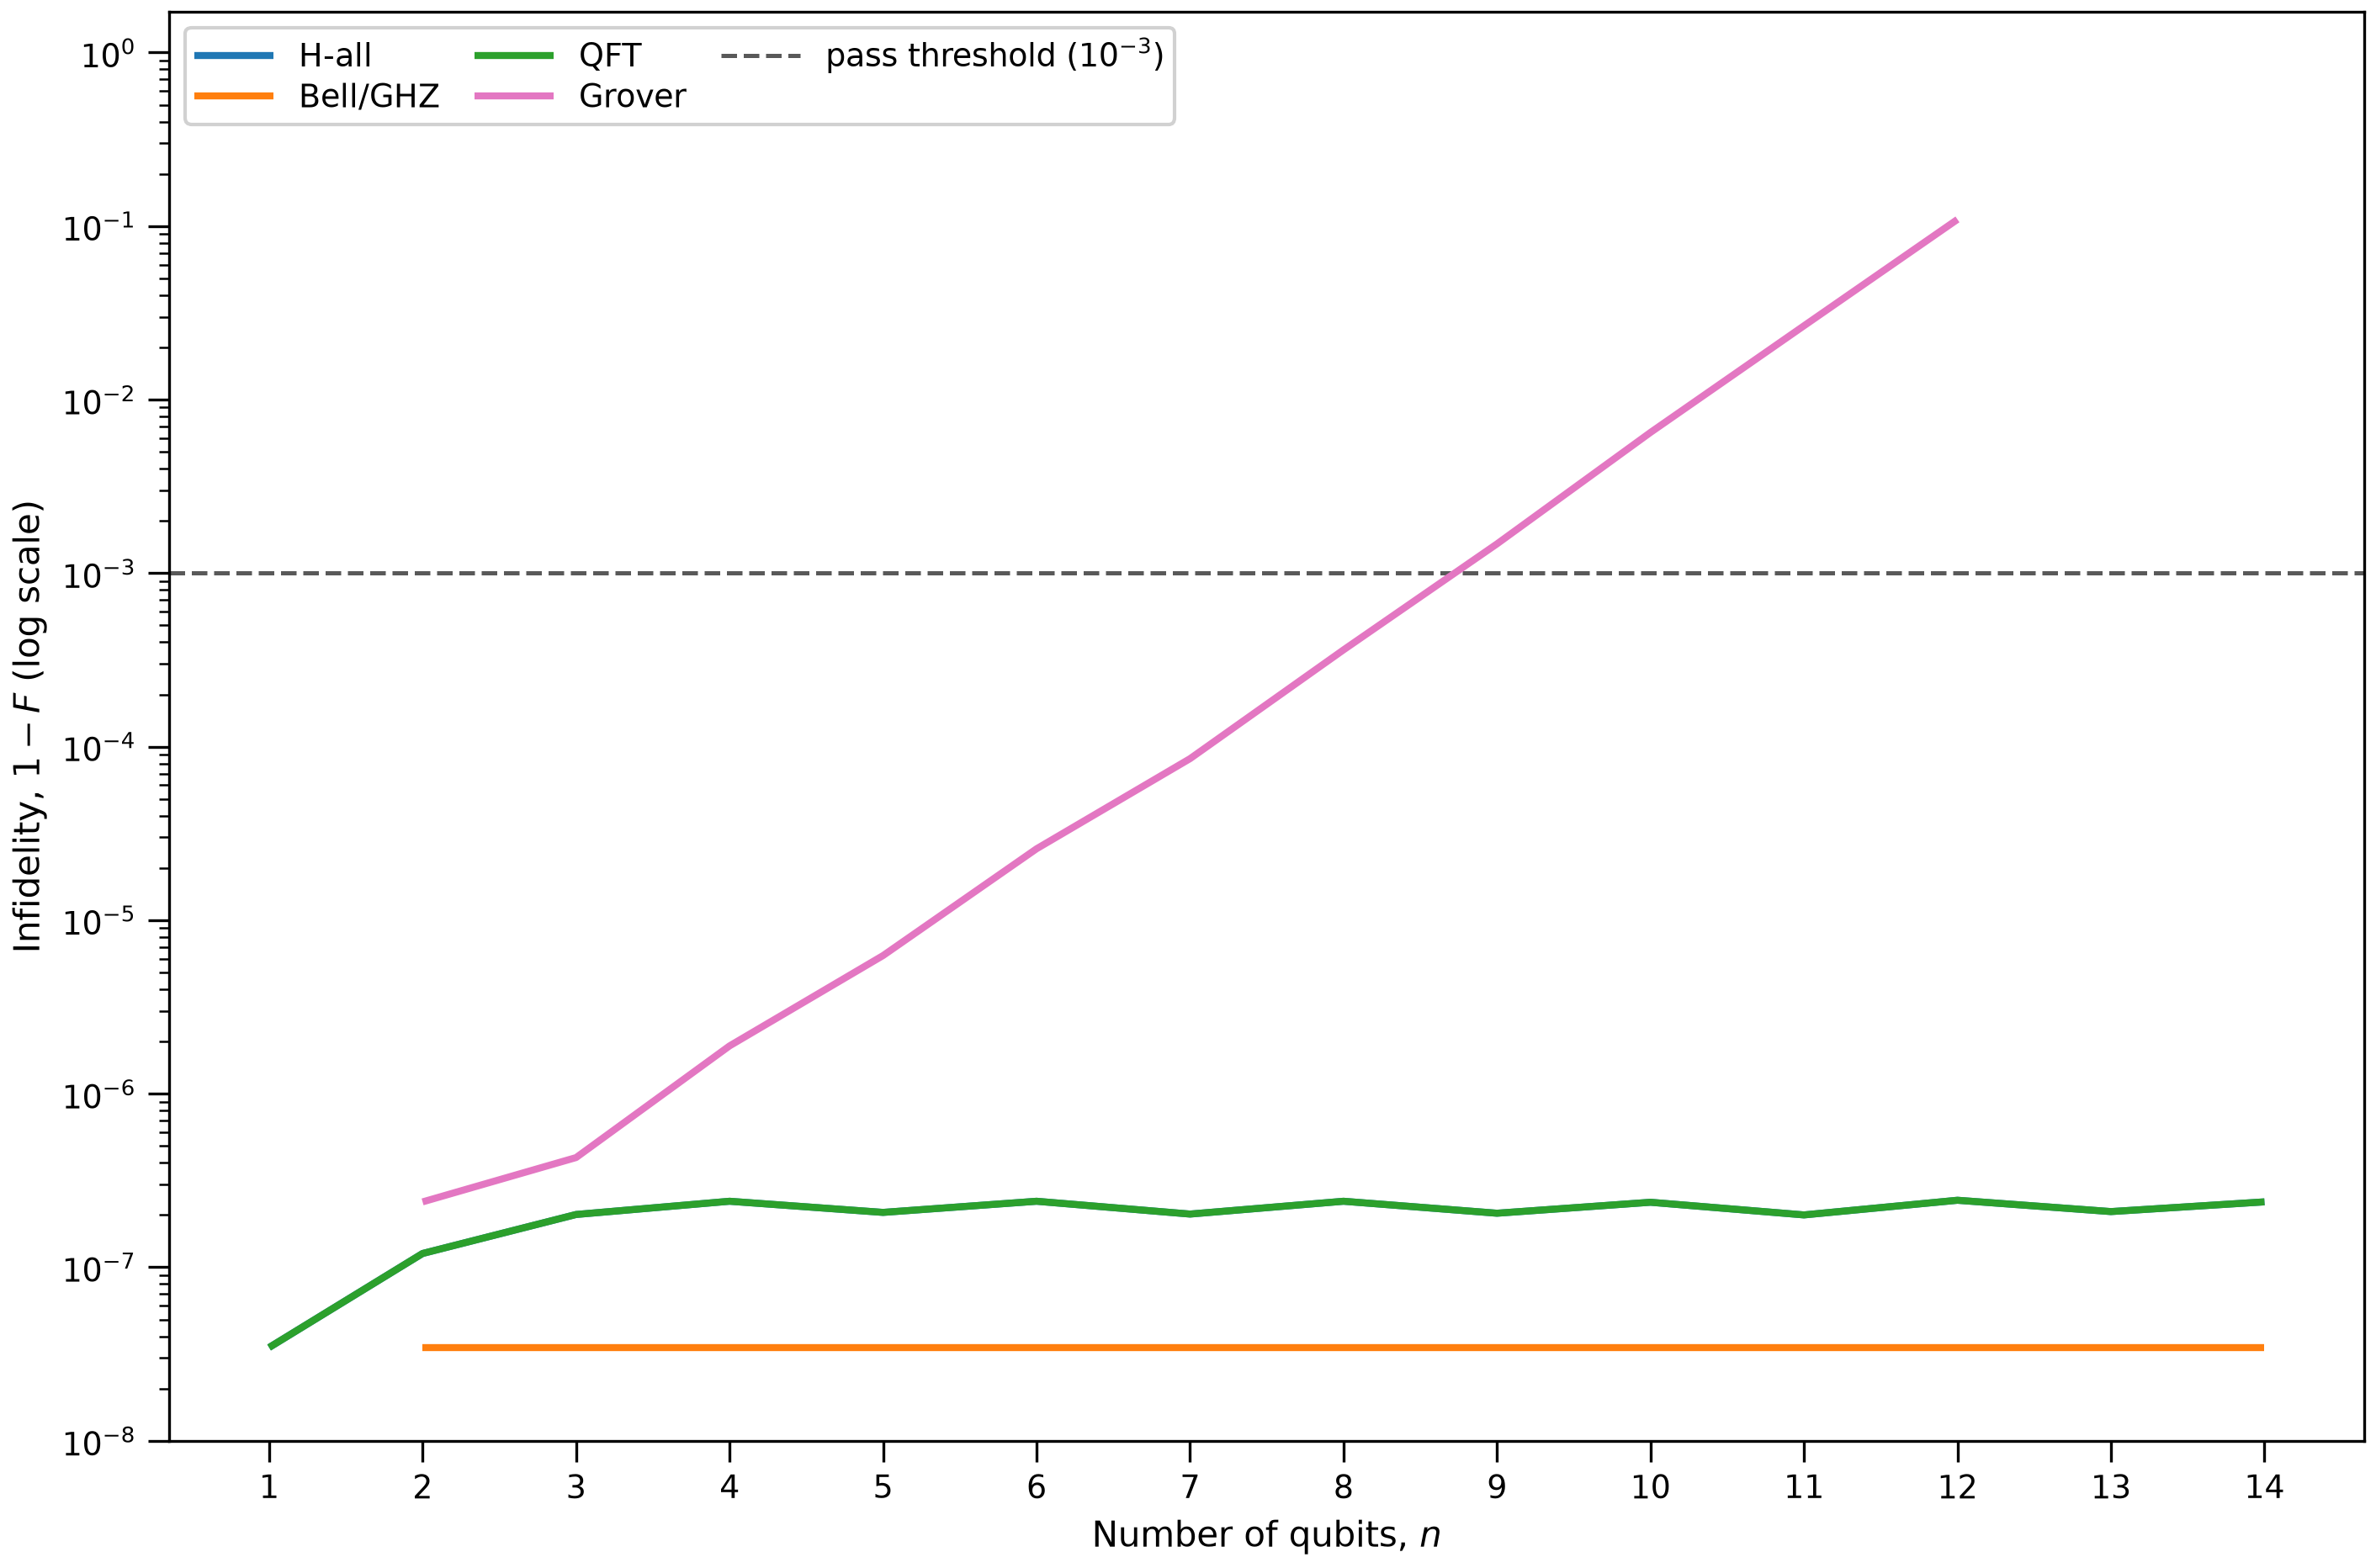
\includegraphics[width=\linewidth]{../data/figures/phase1/phase1_accuracy.png}\\[-1pt]\small (a) Phase~1: float32 accuracy (PC)\end{minipage}\hfill
\begin{minipage}[t]{0.47\textwidth}\centering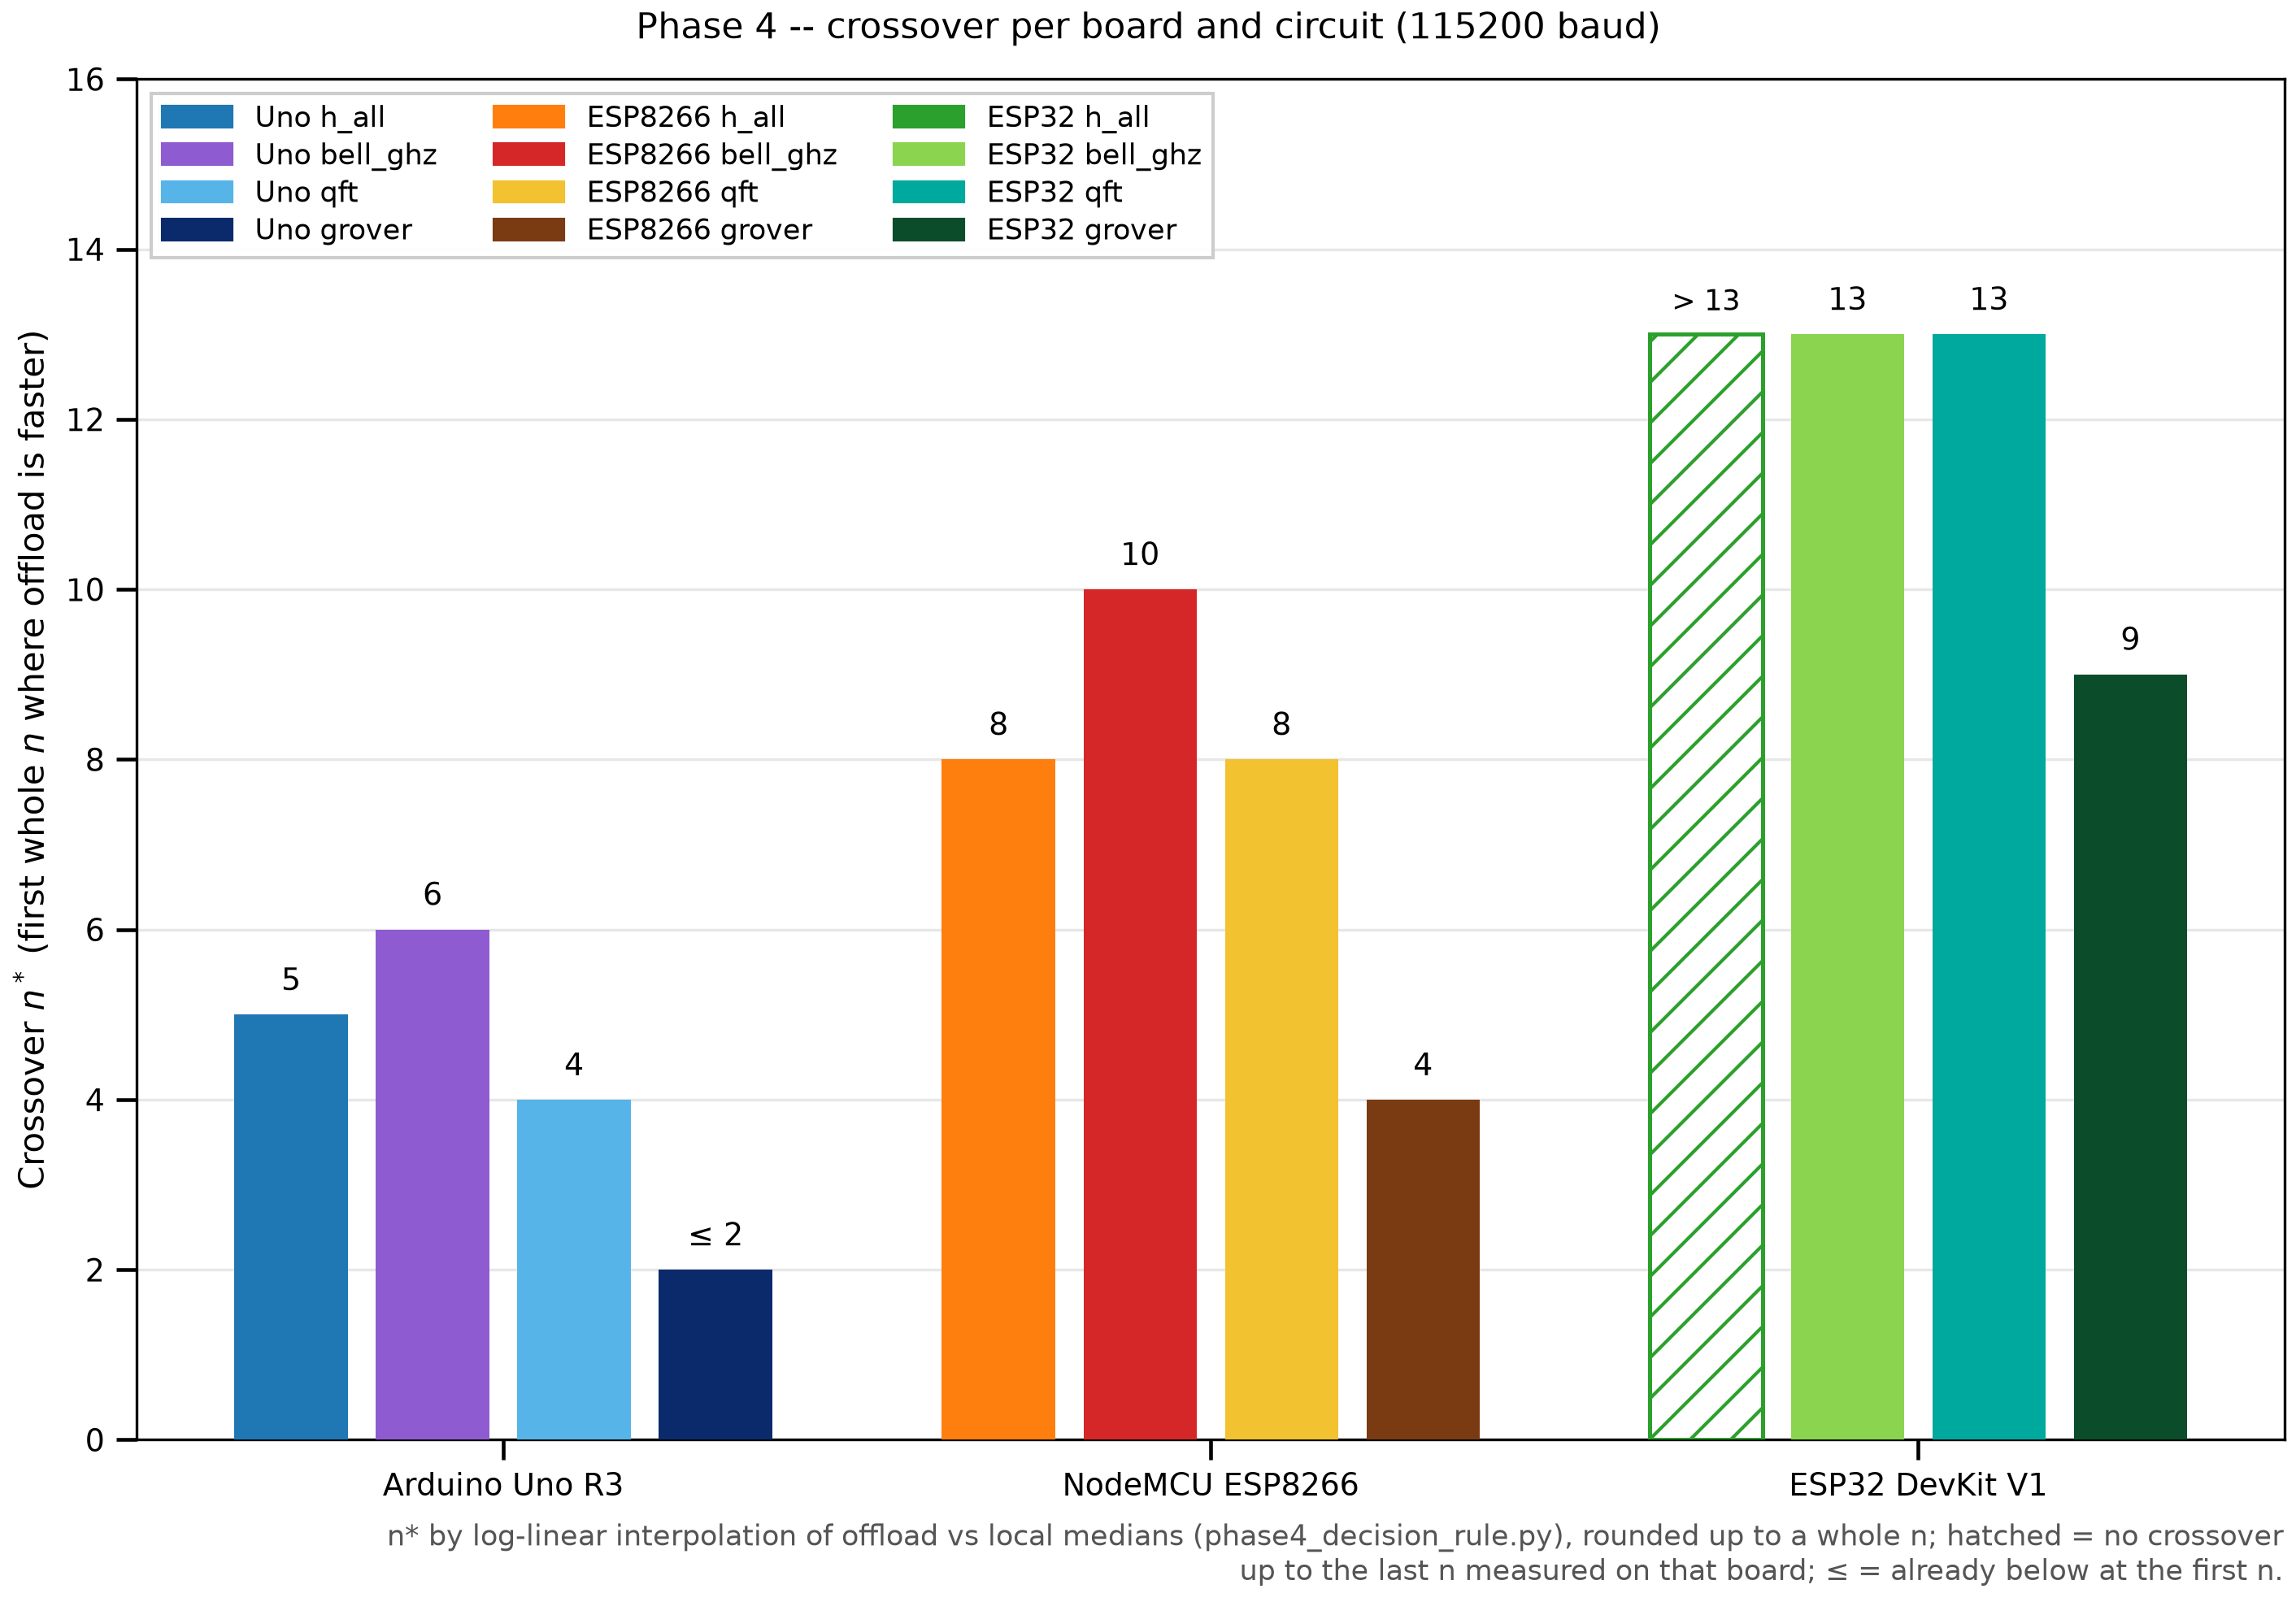
\includegraphics[width=\linewidth]{../data/figures/phase4/all_boards_all_circuits.png}\\[-1pt]\small (b) Phase~4: crossover\end{minipage}
\caption{(a) Phase~1, PC build: infidelity $1-F$ of the float32 simulator against Qiskit Aer versus $n$, without renormalisation, with the $10^{-3}$ acceptance gate dashed; \hall\ is identical to \qft\ and drawn beneath it. (b) Phase~4: the number of qubits at which the Phase~2 and Phase~3 lines cross, rounded up to the first whole $n$ at which offload is faster. It is read from the reference-counter medians with straight segments between measured $n$, so it is not the bracket of Table~\ref{tab:cross}, which uses \texttt{micros()} and the round trip. Circuits whose lines do not cross (Uno \grover, \espB\ \hall) are not drawn.}\label{fig:cross}
\end{figure*}

\begin{figure*}[t]
\centering
\panel{../data/figures/phase2/algorithms/h_all.png}{(a) \hall}\hfill
\panel{../data/figures/phase2/algorithms/bell_ghz.png}{(b) \bell}

\panel{../data/figures/phase2/algorithms/qft.png}{(c) \qft}\hfill
\panel{../data/figures/phase2/algorithms/grover.png}{(d) \grover}
\caption{Phase~2: local execution time per run (reference-counter median, $\mu$s, log scale) versus $n$ for the Uno, \espA\ and \espB\ (blue, orange, green), one panel per circuit. Only points whose counter pair passed the validity rules are drawn, joined by straight segments, so a line can skip an $n$.}\label{fig:loc}
\end{figure*}

\begin{figure*}[t]
\centering
\panel{../data/figures/phase2/timer_vs_counter/circuit/h_all.png}{(a) \hall}\hfill
\panel{../data/figures/phase2/timer_vs_counter/circuit/bell_ghz.png}{(b) \bell}

\panel{../data/figures/phase2/timer_vs_counter/circuit/qft.png}{(c) \qft}\hfill
\panel{../data/figures/phase2/timer_vs_counter/circuit/grover.png}{(d) \grover}
\caption{Phase~2: reference counter against the on-board timer, time per run ($\mu$s, log scale) versus $n$, one panel per circuit, Uno, \espA\ and \espB\ in blue, orange and green. Solid: reference counter (a separate ESP32); dashed: the board's own \texttt{micros()}; shaded: the difference between the two.}\label{fig:p2tc}
\end{figure*}

\begin{figure*}[t]
\centering
\panel{../data/figures/phase4/algorithms/h_all.png}{(a) \hall}\hfill
\panel{../data/figures/phase4/algorithms/bell_ghz.png}{(b) \bell}

\panel{../data/figures/phase4/algorithms/qft.png}{(c) \qft}\hfill
\panel{../data/figures/phase4/algorithms/grover.png}{(d) \grover}
\caption{Phase~4: local (Phase~2) and offload (Phase~3) time per run versus $n$ on the same axes, one panel per circuit, from the reference-counter medians. The point where an offload line crosses the local line of the same board is the crossover of Fig.~\ref{fig:cross}b.}\label{fig:both}
\end{figure*}

\textbf{Float32 accuracy (Phase~1, PC build, Fig.~\ref{fig:cross}a).} \hall, \bell\ and \qft\ pass the \PoneGate\ infidelity gate at every tested $n$ (largest infidelity \PoneMaxHall, \PoneMaxBell, \PoneMaxQft). The raw infidelity of \grover\ passes up to $n=\PoneGroverLastPass$ and fails from $n=\PoneGroverFirstFail$; this is a loss of norm, not a wrong state: the infidelity of the normalised state stays below \DirMaxTwelve\ for $n\le12$. The float32 constant $1/\sqrt2$ (relative error \ConstRelErr) accounts for the loss but over-predicts it by about \LogLossOverPct\,\%. The normalised criterion was chosen after this was understood. The gate itself is the project's own acceptance value, set before the Phase~1 data were collected; it sits well above the float32 rounding of about $10^{-7}$ per operation, and only the last passing $n$ of \grover\ moves when it is changed. A float64 build and Aer both match the closed-form \grover\ state ($\le$\,\DoubleMax\ and $\le$\,\AerMax). Whether the board builds lose norm likewise was not tested.

\textbf{Memory walls.} For \hall, \bell\ and \qft\ the largest working $n$ is \MemOkUno\ (Uno), \MemOkEspLo\ (\espA) and \MemOkEspHi\ (\espB), and the first failure is one qubit higher on every board (Table~\ref{tab:mem}). Eq.~\eqref{eq:mem} reproduces all \MemWallRows\ board--circuit rows when $B$ is the Uno static RAM, the \espA\ free heap and the \espB\ \emph{largest free block} (\MemBEspHi\,B); the \espB\ total free heap (\MemBEspHiTotal\,B) predicts $n=\MemPredEspHiTotal$, one qubit too many, because the failing state of $n=\MemWallEspHi$ needs one contiguous block of \MemStateAtWallEspHi\,B. The test resolves $B$ only to a factor of two, the Uno $B$ comes from the same compiler figure that triggers the overflow (close to circular), and the \espB\ predictor was chosen after the walls were known. \grover\ on the ESP boards stopped at the time cap (\espA\ at $n=\GroverLastNEspLo$, \espB\ at $n=\GroverLastNEspHi$) before any wall; their predicted limits (\GroverPredEspLo, \GroverPredEspHi) are untested.

\begin{table}[t]
\caption{Predicted versus measured memory wall for \hall, \bell, \qft\ ($B$ in bytes, read at $n=2$). ``wrong'': the prediction exceeds the last working $n$.}\label{tab:mem}
\centering\footnotesize
\resizebox{\columnwidth}{!}{\begin{tabular}{@{}llrrrrl@{}}
\toprule
Board & $B$ from & $B$ (B) & Pred. $n_{\max}$ & Last ok & First fail & Evidence \\
\midrule
Uno R3 & static SRAM & 1\,842--1\,848 & 7 & 7 & 8 & build\_overflow \\
ESP8266 & total free heap & 52\,240 & 12 & 12 & 13 & malloc\_failed \\
ESP32 & largest block & 110\,580 & 13 & 13 & 14 & malloc\_failed \\
ESP32 & total free heap & 256\,328 & 14 (wrong) & 13 & 14 & malloc\_failed \\
\bottomrule
\end{tabular}
}
\end{table}

\textbf{Execution time.} On a log axis the non-\grover\ series are roughly straight (Fig.~\ref{fig:loc}), consistent with work $\propto$ gate calls $\times\,2^n$. The held-out scores are: M2 reaches \MapeTwo\,\% MAPE over \NTestTwo\ non-weak points against \MapeOne\,\% for M1, and a constant per board and circuit (M1c) \MapeOneCOne\,\%; per board M1 scores \MapeOneUno, \MapeOneEspLo\ and \MapeOneEspHi\,\% (Uno, \espA, \espB). Clean (firmware class~A only) scores are \MapeTwoClean\,\% (M2) and \MapeOneClean\,\% (M1). The model is not identifiable on the Uno at the primary split (the verdict changes with the held-out size, as a coefficient sits on the non-negativity boundary), \espA\ \grover\ is excluded because its firmware ran a timer interrupt inside the timed region, and M2 was not defined blind with respect to \grover. M2 scores \MapeTwoUno\,\% (Uno), \MapeTwoEspLo\,\% (\espA) and \MapeTwoEspHi\,\% (\espB); without \grover\ in the fit (M2g) it reaches \MapeTwoG\,\%, and the largest error of a single series is Uno \qft\ (\MapeTwoUnoQft\,\%). Over held-out sizes 2--4 M2 stays within \SensTwoAllMin--\SensTwoAllMax\,\% (M1: \SensOneAllTwo--\SensOneAllFour\,\%). M2's constants are fits, not gate costs: the fitted \espA\ CNOT cost corresponds to \CyclesCnotEspLo\ cycles per loop iteration, which is physically impossible.

\textbf{Timer agreement (Fig.~\ref{fig:p2tc}).} On usable counter points the median \texttt{micros()}/counter ratio is \RatioMedUno\ (Uno), \RatioMedEspLo\ (\espA) and \RatioMedEspHi\ (\espB); the \espB\ worst point is \EspHiWorstPct\,\% off. The Uno reads \UnoBelowPct\,\% below the counter, which we interpret, without proof, as a property of the Uno timebase. Of the Phase~2 counter points, \UsableNUno\ of \RecordedNUno\ (Uno), \UsableNEspLo\ of \RecordedNEspLo\ (\espA) and \UsableNEspHi\ of \RecordedNEspHi\ (\espB) pass the validity rules; the counter could not pair most long \espA\ points nor \espB\ \grover\ at $n=12$ (suspected line noise; unverified). This is agreement between two uncalibrated clocks, conditional on the coarse rule R5 added after the data were seen, and it is not documented above \RatioLongSEspLo\,s on the ESP boards.

\textbf{Offload crossover.} The round trip has a floor of \FloorMsUno\,ms (Uno), \FloorMsEspLo\,ms (\espA) and \FloorMsEspHi\,ms (\espB) at $n\le4$, so offload loses at small $n$ and wins once the exponential local time passes it (Fig.~\ref{fig:both}: the round trip is nearly flat except for \grover, whose PC simulation grows; Fig.~\ref{fig:cross}b and Table~\ref{tab:cross}). \CrossBoth\ of \NCross\ board--circuit pairs have a bracket under both bounds; \espB\ \hall\ has none up to $n=13$ under the slow bound, and Uno \grover\ is already faster offloaded at the smallest $n$ under the fast bound. For all four circuits the bracket moves to larger $n$ from Uno to \espA\ to \espB: the faster the board, the later offloading pays (with three boards, speed and link residual of \ResidBoardUno, \ResidBoardEspLo\ and \ResidBoardEspHi\,ms cannot be separated). Read from the reference-counter medians instead (Fig.~\ref{fig:cross}b), the lines cross at $n=5$, 6 and 5 on the Uno (\hall, \bell, \qft), 8, 11, 7 and 4 on the \espA\ (\hall, \bell, \qft, \grover) and 13, 13 and 9 on the \espB\ (\bell, \qft, \grover), each inside or next to the corresponding bracket of Table~\ref{tab:cross}, except Uno \qft\ (5 against the bracket 3--4). Between the two PC bounds the bracket moves by at most \ShiftMax\ measured step in the \ShiftN\ pairs where offload wins under both (identical in \ShiftSame, one step apart in \ShiftOne). \LabNoise\ of the bracket labels are \emph{within noise} and \LabWeak\ have a weak point in or beyond the bracket. The width of the band is the host PC's speed, which varied by a median \SimSpreadMed$\times$ (up to \SimSpreadMax$\times$) between sessions, so the crossover is a property of the pair (board, PC). Beyond the wall only offload exists (Uno to $n=\OffNMaxUno$, \espA\ to \OffNMaxEspLo, \espB\ to \OffNMaxEspHi). Using M2 in Eq.~\eqref{eq:cross}, the predicted bracket equals the measured one in \PredMatchTwo\ of \PredN\ comparisons where M2 is identifiable (M1: \PredMatchOne), is one measured step off in \PredOffOneTwo\ and further off in \PredOffMoreTwo; because local time doubles per qubit while the band is flat, a bracket can match despite a sizeable model error.

\begin{table}[t]
\caption{Crossover brackets: two consecutive measured $n$ between which offload becomes faster and stays faster, for the fast and slow PC bound. $\le2$: faster at the smallest $n$; none: no crossover. $^\dagger$ within noise; $^\ddagger$ weak point in or beyond the bracket.}\label{tab:cross}
\centering\footnotesize
\begin{tabular}{@{}llccc@{}}
\toprule
Board & Circuit & Measured $n$ & Fast PC & Slow PC \\
\midrule
Uno R3 & \hall & 2--7 & 4--5 & 4--5 \\
 & \bell & 2--7 & 5--6 & 6--7$^{\dagger}$ \\
 & \qft & 2--7 & 3--4 & 3--4$^{\dagger}$ \\
 & \grover & 2--7 & $\le$2$^{\dagger}$ & 2--3$^{\dagger}$ \\
\espA & \hall & 2--12 & 7--8$^{\dagger}$ & 7--8 \\
 & \bell & 2--12 & 9--10$^{\dagger}$ & 10--11$^{\dagger}$ \\
 & \qft & 2--12 & 6--7$^{\dagger}$ & 7--8 \\
 & \grover & 2--10 & 3--4$^{\ddagger}$ & 4--5$^{\ddagger}$ \\
\espB & \hall & 2--13 & 12--13$^{\dagger}$ & none$^{\dagger}$ \\
 & \bell & 2--13 & 12--13 & 12--13 \\
 & \qft & 2--13 & 11--12 & 12--13 \\
 & \grover & 2--12 & 8--9$^{\ddagger}$ & 9--10$^{\ddagger}$ \\
\bottomrule
\end{tabular}
\end{table}

\textbf{Reproducibility.} Phase~2 timer medians of \ReproPtwoN\ points measured in more than one session (all \grover\ on the ESP boards) differ by at most \ReproPtwoMaxPct\,\%. Phase~3 round trips of \ReproPthreeN\ \espA\ points differ between the original and the repeat session by a median \ReproPthreeE\,\% (maximum \ReproPthreeEMax\,\%), mostly through the PC simulation time (median \ReproPthreeSim\,\%), which the band of Table~\ref{tab:cross} covers; the cause of the PC speed change was not recorded.

\section{Discussion and Limitations}\label{sec:disc}
\textbf{What limits each board.} On the Uno the limit is the \MemSramUno\,B SRAM: the state of $n=\MemWallUno$ no longer fits next to \MemOverheadUnoMin--\MemOverheadUnoMax\,B of static use. On the \espA\ it is the free heap and on the \espB\ the largest contiguous block. Memory needs one low-$n$ read; time needs a model, and per-gate-kind costs lower the held-out error from \MapeOne\,\% to \MapeTwo\,\% but remain fits. Offload has a floor of a few milliseconds (serial link, USB latency, host scheduling and the Aer build and run; the split was not tested), so local execution on a fast board wins below the crossover and is impossible beyond the wall.

\textbf{Scope.} One unit per board, one PC and one baud rate were measured; how the brackets move with another PC or link is not tested. There are no board-level correctness data, and Phase~3 compares its single sampled outcome with nothing. No hash of the flashed binary was recorded, and firmware versions were classified from the source diff.

\textbf{Measurement.} The counter is uncalibrated and its offset of \SelfTestLo--\SelfTestHi\,\textmu s cannot be split between generator and counter. The Uno timer resolves \UnoResUs\,\textmu s, the ESP timers \EspResUs\,\textmu s. In Eq.~\eqref{eq:off} the residual absorbs the error of subtracting two medians, so it is bookkeeping, not a measurement. The \espA\ Phase~3 data come from one repeat session, and two \espB\ \grover\ points contain repeated rows (\DupNineIndep\ and \DupTenIndep\ independent of \DupNineRows\ recorded rows), of which only the independent ones are used.

\textbf{Post-hoc choices.} The following were set after data or scores were seen: the weak-point rule, the firmware classes, the identifiability rule, the primary Phase~1 criterion, the selection of the session that supplies each point, counter rule R5, the choice of the memory predictor per board, the band-and-bracket design of the crossover and the predicted-crossover comparison. The split (largest three $n$) and the \ModelFloorUs\,\textmu s floor were fixed before scoring by the authors' record, which cannot be verified from the commit history. The effect of the rules together was not split.

\section{Conclusion}
Memory ends \hall, \bell\ and \qft\ at $n=\MemWallUno$, \MemWallEspLo\ and \MemWallEspHi\ on the Uno, \espA\ and \espB, while \grover\ on the ESP boards stopped at the time cap. The wall is consistent with one low-$n$ memory read, held-out time is predicted to about \MapeTwoClean\,\% with a model that is a fit, not a gate cost, and offload overtakes local execution within brackets of measured $n$ that depend on the host PC. All numbers and figures are regenerated from the raw CSVs by one command; the repository link is withheld for blind review.

\bibliographystyle{IEEEtran}
\bibliography{../paper/refs}
\end{document}
